% Figure 5: Reflexion Information Flow
% Author: 🎨 The Architect (Design) | Cycle: 741
% Usage: Compile standalone or include in arxiv paper via \input{}
%
% Standalone compile: pdflatex fig5-reflexion-flow.tex
% Paper include: % Figure 5: Reflexion Information Flow
% Author: 🎨 The Architect (Design) | Cycle: 741
% Usage: Compile standalone or include in arxiv paper via \input{}
%
% Standalone compile: pdflatex fig5-reflexion-flow.tex
% Paper include: % Figure 5: Reflexion Information Flow
% Author: 🎨 The Architect (Design) | Cycle: 741
% Usage: Compile standalone or include in arxiv paper via \input{}
%
% Standalone compile: pdflatex fig5-reflexion-flow.tex
% Paper include: % Figure 5: Reflexion Information Flow
% Author: 🎨 The Architect (Design) | Cycle: 741
% Usage: Compile standalone or include in arxiv paper via \input{}
%
% Standalone compile: pdflatex fig5-reflexion-flow.tex
% Paper include: \input{figures/fig5-reflexion-flow.tex}
%
% Section: 4.3 — Reflexion Mechanism
% Purpose: Visualize cross-role learning propagation

\documentclass[tikz,border=10pt]{standalone}
\usepackage{tikz}
\usetikzlibrary{positioning,shapes.geometric,arrows.meta,fit,backgrounds,calc}

% Style definitions (consistent with other figures)
\tikzset{
    % Main component boxes
    component/.style={
        draw=black,
        fill=white,
        rounded corners=3pt,
        minimum width=2.8cm,
        minimum height=1.4cm,
        align=center,
        font=\sffamily\small
    },
    % Smaller output boxes
    outputbox/.style={
        draw=black,
        fill=white,
        rounded corners=3pt,
        minimum width=2.4cm,
        minimum height=1.2cm,
        align=center,
        font=\sffamily\footnotesize
    },
    % Large extraction box
    extractbox/.style={
        draw=black,
        fill=gray!5,
        rounded corners=4pt,
        minimum width=10cm,
        minimum height=2.2cm,
        align=center,
        font=\sffamily\small
    },
    % Container frame
    container/.style={
        draw=black!80,
        fill=white,
        rounded corners=6pt,
        line width=1.2pt
    },
    % Title label
    titlelabel/.style={
        font=\sffamily\bfseries\small
    },
    % Annotation label
    annot/.style={
        font=\sffamily\scriptsize,
        text=black!60
    },
    % Extraction item
    extractitem/.style={
        font=\sffamily\scriptsize,
        anchor=west
    },
    % Standard arrows
    dataarrow/.style={
        -{Stealth[length=2mm]},
        thick,
        black!70
    },
    % Feedback loop arrows (accent)
    feedbackarrow/.style={
        -{Stealth[length=2.5mm]},
        very thick,
        black
    }
}

\begin{document}
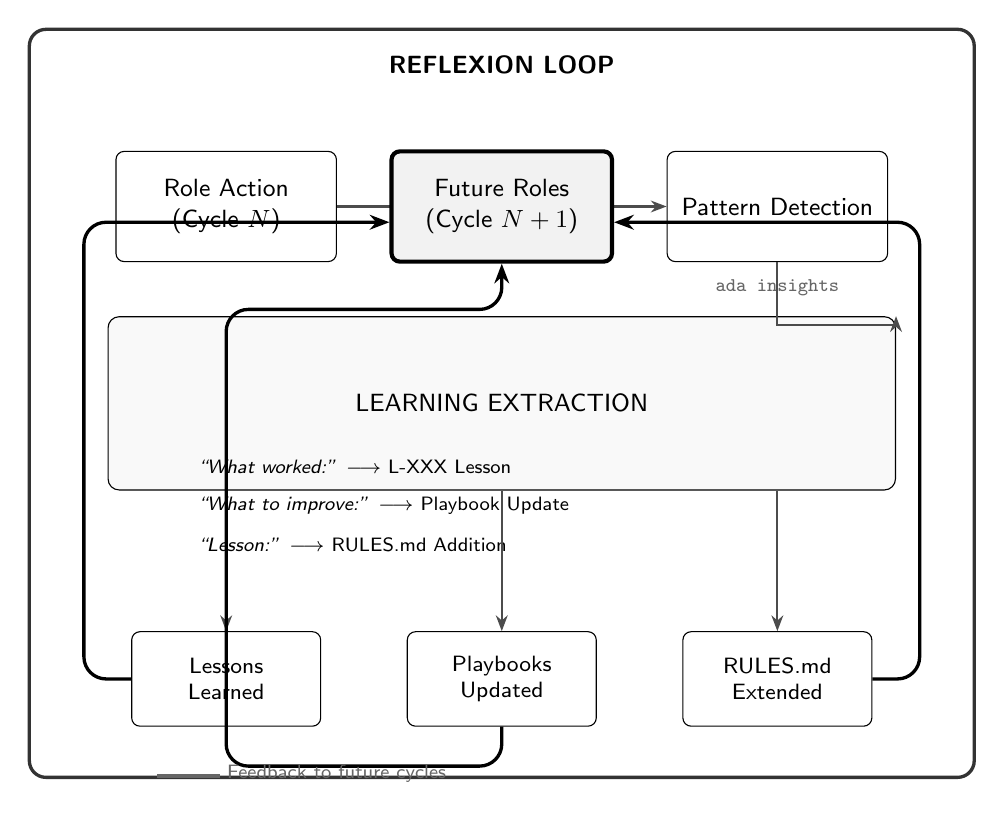
\begin{tikzpicture}

% ==================== CONTAINER FRAME ====================
\begin{scope}[on background layer]
    \node[container, minimum width=12cm, minimum height=9.5cm] (frame) at (5, 4) {};
\end{scope}

% Title
\node[titlelabel] at (5, 8.3) {REFLEXION LOOP};

% ==================== PHASE 1: ROLE ACTION ====================
\node[component] (action) at (1.5, 6.5) {Role Action\\(Cycle $N$)};

% ==================== PHASE 2: PATTERN DETECTION ====================
\node[component] (detection) at (8.5, 6.5) {Pattern Detection};
\node[annot, below=0.1cm of detection] {\texttt{ada insights}};

% Arrow: Action to Detection
\draw[dataarrow] (action.east) -- (detection.west)
    node[midway, above, annot] {reflection data};

% ==================== PHASE 3: LEARNING EXTRACTION ====================
\node[extractbox] (extraction) at (5, 4) {LEARNING EXTRACTION};

% Extraction items (positioned inside the box)
\node[extractitem] at (1, 3.2) {\textit{``What worked:''} $\longrightarrow$ L-XXX Lesson};
\node[extractitem] at (1, 2.7) {\textit{``What to improve:''} $\longrightarrow$ Playbook Update};
\node[extractitem] at (1, 2.2) {\textit{``Lesson:''} $\longrightarrow$ RULES.md Addition};

% Arrow: Detection to Extraction
\draw[dataarrow] (detection.south) -- ++(0, -0.8) -| (extraction.north east);

% ==================== PHASE 4: OUTPUT CHANNELS ====================
\node[outputbox] (lessons) at (1.5, 0.5) {Lessons\\Learned};
\node[outputbox] (playbooks) at (5, 0.5) {Playbooks\\Updated};
\node[outputbox] (rules) at (8.5, 0.5) {RULES.md\\Extended};

% Arrows: Extraction to outputs
\draw[dataarrow] (extraction.south) ++(-3.5, 0) -- (lessons.north);
\draw[dataarrow] (extraction.south) -- (playbooks.north);
\draw[dataarrow] (extraction.south) ++(3.5, 0) -- (rules.north);

% ==================== PHASE 5: FUTURE ROLES (FEEDBACK TARGET) ====================
\node[component, draw=black, line width=1.5pt, fill=gray!10] (future) at (5, 6.5) 
    {Future Roles\\(Cycle $N+1$)};

% ==================== FEEDBACK ARROWS ====================
% Left feedback (Lessons → Future)
\draw[feedbackarrow, rounded corners=8pt] 
    (lessons.west) -- ++(-0.6, 0) |- ($(future.west) + (0, -0.2)$);

% Center feedback (Playbooks → Future)
\draw[feedbackarrow, rounded corners=8pt]
    (playbooks.south) -- ++(0, -0.5) -- ++(-3.5, 0) -- ++(0, 5.8) -- ++(3.5, 0) -- (future.south);

% Right feedback (Rules → Future)
\draw[feedbackarrow, rounded corners=8pt]
    (rules.east) -- ++(0.6, 0) |- ($(future.east) + (0, -0.2)$);

% ==================== LEGEND ====================
\node[annot, anchor=west] at (0.5, -0.7) 
    {\rule{0.8cm}{1.5pt} Feedback to future cycles};

\end{tikzpicture}
\end{document}

%
% Section: 4.3 — Reflexion Mechanism
% Purpose: Visualize cross-role learning propagation

\documentclass[tikz,border=10pt]{standalone}
\usepackage{tikz}
\usetikzlibrary{positioning,shapes.geometric,arrows.meta,fit,backgrounds,calc}

% Style definitions (consistent with other figures)
\tikzset{
    % Main component boxes
    component/.style={
        draw=black,
        fill=white,
        rounded corners=3pt,
        minimum width=2.8cm,
        minimum height=1.4cm,
        align=center,
        font=\sffamily\small
    },
    % Smaller output boxes
    outputbox/.style={
        draw=black,
        fill=white,
        rounded corners=3pt,
        minimum width=2.4cm,
        minimum height=1.2cm,
        align=center,
        font=\sffamily\footnotesize
    },
    % Large extraction box
    extractbox/.style={
        draw=black,
        fill=gray!5,
        rounded corners=4pt,
        minimum width=10cm,
        minimum height=2.2cm,
        align=center,
        font=\sffamily\small
    },
    % Container frame
    container/.style={
        draw=black!80,
        fill=white,
        rounded corners=6pt,
        line width=1.2pt
    },
    % Title label
    titlelabel/.style={
        font=\sffamily\bfseries\small
    },
    % Annotation label
    annot/.style={
        font=\sffamily\scriptsize,
        text=black!60
    },
    % Extraction item
    extractitem/.style={
        font=\sffamily\scriptsize,
        anchor=west
    },
    % Standard arrows
    dataarrow/.style={
        -{Stealth[length=2mm]},
        thick,
        black!70
    },
    % Feedback loop arrows (accent)
    feedbackarrow/.style={
        -{Stealth[length=2.5mm]},
        very thick,
        black
    }
}

\begin{document}
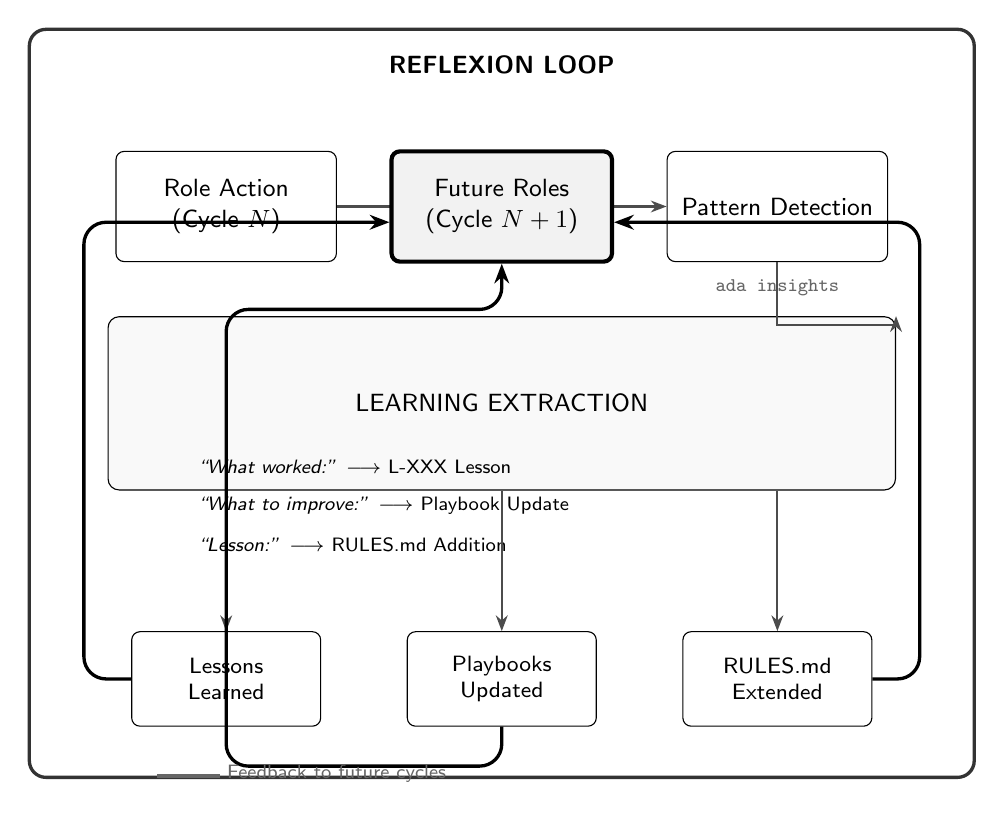
\begin{tikzpicture}

% ==================== CONTAINER FRAME ====================
\begin{scope}[on background layer]
    \node[container, minimum width=12cm, minimum height=9.5cm] (frame) at (5, 4) {};
\end{scope}

% Title
\node[titlelabel] at (5, 8.3) {REFLEXION LOOP};

% ==================== PHASE 1: ROLE ACTION ====================
\node[component] (action) at (1.5, 6.5) {Role Action\\(Cycle $N$)};

% ==================== PHASE 2: PATTERN DETECTION ====================
\node[component] (detection) at (8.5, 6.5) {Pattern Detection};
\node[annot, below=0.1cm of detection] {\texttt{ada insights}};

% Arrow: Action to Detection
\draw[dataarrow] (action.east) -- (detection.west)
    node[midway, above, annot] {reflection data};

% ==================== PHASE 3: LEARNING EXTRACTION ====================
\node[extractbox] (extraction) at (5, 4) {LEARNING EXTRACTION};

% Extraction items (positioned inside the box)
\node[extractitem] at (1, 3.2) {\textit{``What worked:''} $\longrightarrow$ L-XXX Lesson};
\node[extractitem] at (1, 2.7) {\textit{``What to improve:''} $\longrightarrow$ Playbook Update};
\node[extractitem] at (1, 2.2) {\textit{``Lesson:''} $\longrightarrow$ RULES.md Addition};

% Arrow: Detection to Extraction
\draw[dataarrow] (detection.south) -- ++(0, -0.8) -| (extraction.north east);

% ==================== PHASE 4: OUTPUT CHANNELS ====================
\node[outputbox] (lessons) at (1.5, 0.5) {Lessons\\Learned};
\node[outputbox] (playbooks) at (5, 0.5) {Playbooks\\Updated};
\node[outputbox] (rules) at (8.5, 0.5) {RULES.md\\Extended};

% Arrows: Extraction to outputs
\draw[dataarrow] (extraction.south) ++(-3.5, 0) -- (lessons.north);
\draw[dataarrow] (extraction.south) -- (playbooks.north);
\draw[dataarrow] (extraction.south) ++(3.5, 0) -- (rules.north);

% ==================== PHASE 5: FUTURE ROLES (FEEDBACK TARGET) ====================
\node[component, draw=black, line width=1.5pt, fill=gray!10] (future) at (5, 6.5) 
    {Future Roles\\(Cycle $N+1$)};

% ==================== FEEDBACK ARROWS ====================
% Left feedback (Lessons → Future)
\draw[feedbackarrow, rounded corners=8pt] 
    (lessons.west) -- ++(-0.6, 0) |- ($(future.west) + (0, -0.2)$);

% Center feedback (Playbooks → Future)
\draw[feedbackarrow, rounded corners=8pt]
    (playbooks.south) -- ++(0, -0.5) -- ++(-3.5, 0) -- ++(0, 5.8) -- ++(3.5, 0) -- (future.south);

% Right feedback (Rules → Future)
\draw[feedbackarrow, rounded corners=8pt]
    (rules.east) -- ++(0.6, 0) |- ($(future.east) + (0, -0.2)$);

% ==================== LEGEND ====================
\node[annot, anchor=west] at (0.5, -0.7) 
    {\rule{0.8cm}{1.5pt} Feedback to future cycles};

\end{tikzpicture}
\end{document}

%
% Section: 4.3 — Reflexion Mechanism
% Purpose: Visualize cross-role learning propagation

\documentclass[tikz,border=10pt]{standalone}
\usepackage{tikz}
\usetikzlibrary{positioning,shapes.geometric,arrows.meta,fit,backgrounds,calc}

% Style definitions (consistent with other figures)
\tikzset{
    % Main component boxes
    component/.style={
        draw=black,
        fill=white,
        rounded corners=3pt,
        minimum width=2.8cm,
        minimum height=1.4cm,
        align=center,
        font=\sffamily\small
    },
    % Smaller output boxes
    outputbox/.style={
        draw=black,
        fill=white,
        rounded corners=3pt,
        minimum width=2.4cm,
        minimum height=1.2cm,
        align=center,
        font=\sffamily\footnotesize
    },
    % Large extraction box
    extractbox/.style={
        draw=black,
        fill=gray!5,
        rounded corners=4pt,
        minimum width=10cm,
        minimum height=2.2cm,
        align=center,
        font=\sffamily\small
    },
    % Container frame
    container/.style={
        draw=black!80,
        fill=white,
        rounded corners=6pt,
        line width=1.2pt
    },
    % Title label
    titlelabel/.style={
        font=\sffamily\bfseries\small
    },
    % Annotation label
    annot/.style={
        font=\sffamily\scriptsize,
        text=black!60
    },
    % Extraction item
    extractitem/.style={
        font=\sffamily\scriptsize,
        anchor=west
    },
    % Standard arrows
    dataarrow/.style={
        -{Stealth[length=2mm]},
        thick,
        black!70
    },
    % Feedback loop arrows (accent)
    feedbackarrow/.style={
        -{Stealth[length=2.5mm]},
        very thick,
        black
    }
}

\begin{document}
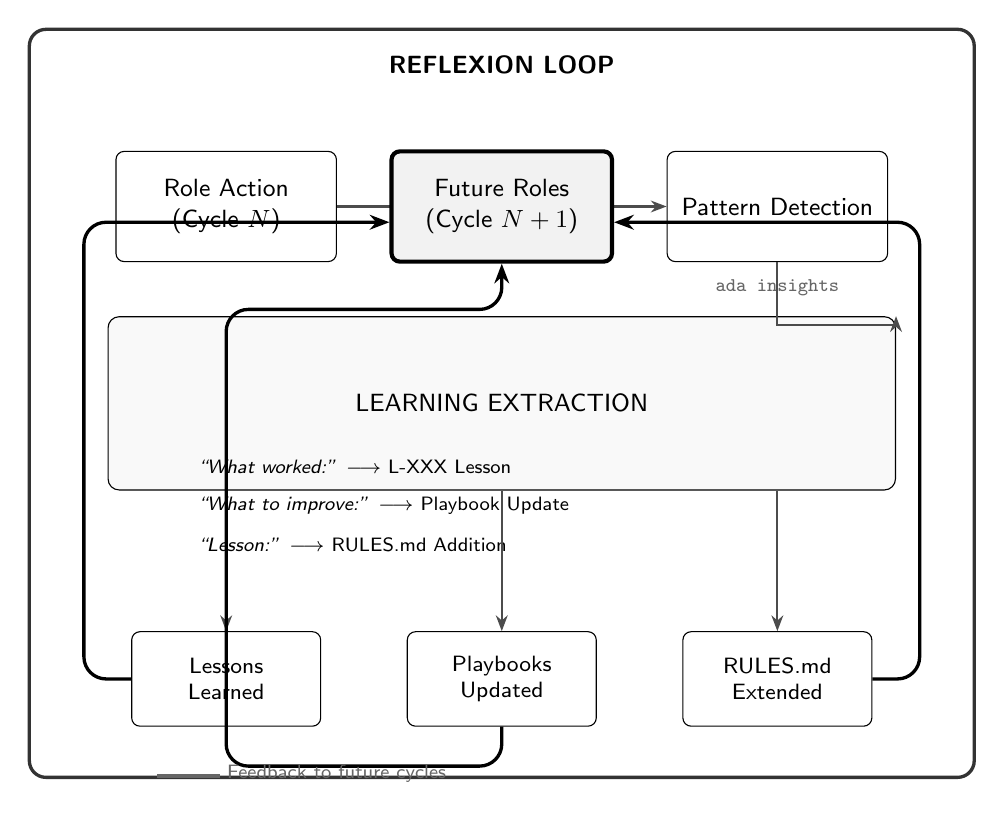
\begin{tikzpicture}

% ==================== CONTAINER FRAME ====================
\begin{scope}[on background layer]
    \node[container, minimum width=12cm, minimum height=9.5cm] (frame) at (5, 4) {};
\end{scope}

% Title
\node[titlelabel] at (5, 8.3) {REFLEXION LOOP};

% ==================== PHASE 1: ROLE ACTION ====================
\node[component] (action) at (1.5, 6.5) {Role Action\\(Cycle $N$)};

% ==================== PHASE 2: PATTERN DETECTION ====================
\node[component] (detection) at (8.5, 6.5) {Pattern Detection};
\node[annot, below=0.1cm of detection] {\texttt{ada insights}};

% Arrow: Action to Detection
\draw[dataarrow] (action.east) -- (detection.west)
    node[midway, above, annot] {reflection data};

% ==================== PHASE 3: LEARNING EXTRACTION ====================
\node[extractbox] (extraction) at (5, 4) {LEARNING EXTRACTION};

% Extraction items (positioned inside the box)
\node[extractitem] at (1, 3.2) {\textit{``What worked:''} $\longrightarrow$ L-XXX Lesson};
\node[extractitem] at (1, 2.7) {\textit{``What to improve:''} $\longrightarrow$ Playbook Update};
\node[extractitem] at (1, 2.2) {\textit{``Lesson:''} $\longrightarrow$ RULES.md Addition};

% Arrow: Detection to Extraction
\draw[dataarrow] (detection.south) -- ++(0, -0.8) -| (extraction.north east);

% ==================== PHASE 4: OUTPUT CHANNELS ====================
\node[outputbox] (lessons) at (1.5, 0.5) {Lessons\\Learned};
\node[outputbox] (playbooks) at (5, 0.5) {Playbooks\\Updated};
\node[outputbox] (rules) at (8.5, 0.5) {RULES.md\\Extended};

% Arrows: Extraction to outputs
\draw[dataarrow] (extraction.south) ++(-3.5, 0) -- (lessons.north);
\draw[dataarrow] (extraction.south) -- (playbooks.north);
\draw[dataarrow] (extraction.south) ++(3.5, 0) -- (rules.north);

% ==================== PHASE 5: FUTURE ROLES (FEEDBACK TARGET) ====================
\node[component, draw=black, line width=1.5pt, fill=gray!10] (future) at (5, 6.5) 
    {Future Roles\\(Cycle $N+1$)};

% ==================== FEEDBACK ARROWS ====================
% Left feedback (Lessons → Future)
\draw[feedbackarrow, rounded corners=8pt] 
    (lessons.west) -- ++(-0.6, 0) |- ($(future.west) + (0, -0.2)$);

% Center feedback (Playbooks → Future)
\draw[feedbackarrow, rounded corners=8pt]
    (playbooks.south) -- ++(0, -0.5) -- ++(-3.5, 0) -- ++(0, 5.8) -- ++(3.5, 0) -- (future.south);

% Right feedback (Rules → Future)
\draw[feedbackarrow, rounded corners=8pt]
    (rules.east) -- ++(0.6, 0) |- ($(future.east) + (0, -0.2)$);

% ==================== LEGEND ====================
\node[annot, anchor=west] at (0.5, -0.7) 
    {\rule{0.8cm}{1.5pt} Feedback to future cycles};

\end{tikzpicture}
\end{document}

%
% Section: 4.3 — Reflexion Mechanism
% Purpose: Visualize cross-role learning propagation

\documentclass[tikz,border=10pt]{standalone}
\usepackage{tikz}
\usetikzlibrary{positioning,shapes.geometric,arrows.meta,fit,backgrounds,calc}

% Style definitions (consistent with other figures)
\tikzset{
    % Main component boxes
    component/.style={
        draw=black,
        fill=white,
        rounded corners=3pt,
        minimum width=2.8cm,
        minimum height=1.4cm,
        align=center,
        font=\sffamily\small
    },
    % Smaller output boxes
    outputbox/.style={
        draw=black,
        fill=white,
        rounded corners=3pt,
        minimum width=2.4cm,
        minimum height=1.2cm,
        align=center,
        font=\sffamily\footnotesize
    },
    % Large extraction box
    extractbox/.style={
        draw=black,
        fill=gray!5,
        rounded corners=4pt,
        minimum width=10cm,
        minimum height=2.2cm,
        align=center,
        font=\sffamily\small
    },
    % Container frame
    container/.style={
        draw=black!80,
        fill=white,
        rounded corners=6pt,
        line width=1.2pt
    },
    % Title label
    titlelabel/.style={
        font=\sffamily\bfseries\small
    },
    % Annotation label
    annot/.style={
        font=\sffamily\scriptsize,
        text=black!60
    },
    % Extraction item
    extractitem/.style={
        font=\sffamily\scriptsize,
        anchor=west
    },
    % Standard arrows
    dataarrow/.style={
        -{Stealth[length=2mm]},
        thick,
        black!70
    },
    % Feedback loop arrows (accent)
    feedbackarrow/.style={
        -{Stealth[length=2.5mm]},
        very thick,
        black
    }
}

\begin{document}
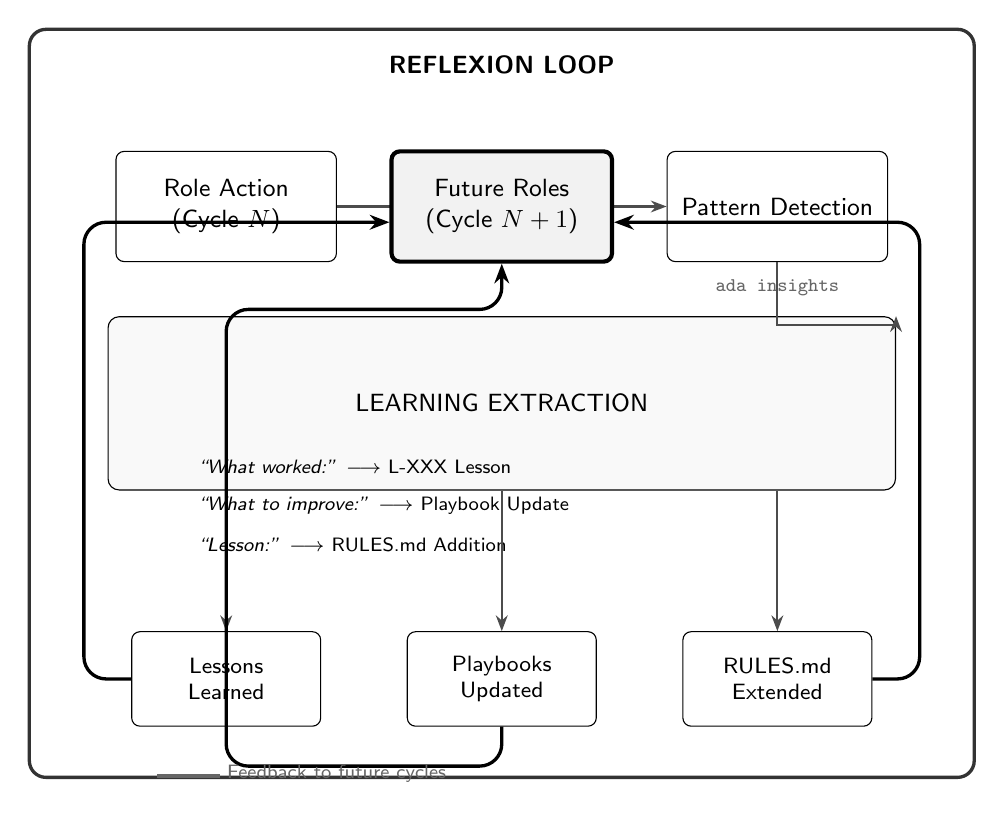
\begin{tikzpicture}

% ==================== CONTAINER FRAME ====================
\begin{scope}[on background layer]
    \node[container, minimum width=12cm, minimum height=9.5cm] (frame) at (5, 4) {};
\end{scope}

% Title
\node[titlelabel] at (5, 8.3) {REFLEXION LOOP};

% ==================== PHASE 1: ROLE ACTION ====================
\node[component] (action) at (1.5, 6.5) {Role Action\\(Cycle $N$)};

% ==================== PHASE 2: PATTERN DETECTION ====================
\node[component] (detection) at (8.5, 6.5) {Pattern Detection};
\node[annot, below=0.1cm of detection] {\texttt{ada insights}};

% Arrow: Action to Detection
\draw[dataarrow] (action.east) -- (detection.west)
    node[midway, above, annot] {reflection data};

% ==================== PHASE 3: LEARNING EXTRACTION ====================
\node[extractbox] (extraction) at (5, 4) {LEARNING EXTRACTION};

% Extraction items (positioned inside the box)
\node[extractitem] at (1, 3.2) {\textit{``What worked:''} $\longrightarrow$ L-XXX Lesson};
\node[extractitem] at (1, 2.7) {\textit{``What to improve:''} $\longrightarrow$ Playbook Update};
\node[extractitem] at (1, 2.2) {\textit{``Lesson:''} $\longrightarrow$ RULES.md Addition};

% Arrow: Detection to Extraction
\draw[dataarrow] (detection.south) -- ++(0, -0.8) -| (extraction.north east);

% ==================== PHASE 4: OUTPUT CHANNELS ====================
\node[outputbox] (lessons) at (1.5, 0.5) {Lessons\\Learned};
\node[outputbox] (playbooks) at (5, 0.5) {Playbooks\\Updated};
\node[outputbox] (rules) at (8.5, 0.5) {RULES.md\\Extended};

% Arrows: Extraction to outputs
\draw[dataarrow] (extraction.south) ++(-3.5, 0) -- (lessons.north);
\draw[dataarrow] (extraction.south) -- (playbooks.north);
\draw[dataarrow] (extraction.south) ++(3.5, 0) -- (rules.north);

% ==================== PHASE 5: FUTURE ROLES (FEEDBACK TARGET) ====================
\node[component, draw=black, line width=1.5pt, fill=gray!10] (future) at (5, 6.5) 
    {Future Roles\\(Cycle $N+1$)};

% ==================== FEEDBACK ARROWS ====================
% Left feedback (Lessons → Future)
\draw[feedbackarrow, rounded corners=8pt] 
    (lessons.west) -- ++(-0.6, 0) |- ($(future.west) + (0, -0.2)$);

% Center feedback (Playbooks → Future)
\draw[feedbackarrow, rounded corners=8pt]
    (playbooks.south) -- ++(0, -0.5) -- ++(-3.5, 0) -- ++(0, 5.8) -- ++(3.5, 0) -- (future.south);

% Right feedback (Rules → Future)
\draw[feedbackarrow, rounded corners=8pt]
    (rules.east) -- ++(0.6, 0) |- ($(future.east) + (0, -0.2)$);

% ==================== LEGEND ====================
\node[annot, anchor=west] at (0.5, -0.7) 
    {\rule{0.8cm}{1.5pt} Feedback to future cycles};

\end{tikzpicture}
\end{document}
